\chapter{Análisis del modelo aplicado a un central solar termoeléctrica real}
\label{analisis-central}

En este capítulo pretendemos emplear nuestro programa de simulación en un análisis del estado del campo solar de una planta termosolar real. Puesto que la simulación de sistemas externos al campo solar queda fuera de nuestro alcance, nos centraremos en los datos referentes al campo solar. En concreto, contrastaremos, para cada  hora del año, qué potencia térmica se estaba extrayendo del campo, independientemente de las causas operativas que condicionasen el funcionamiento del campo cada momento. Nuestro objetivo es comprobar si nuestra herramienta puede ser útil de cara estimar el estado global de rendimiento del campo, midiendo de alguna manera su desviación respecto a lo esperado. Realizaremos la simulación a partir de datos reales (meteorológicos y de generación) de una central termosolar, comparando el salto térmico real con el simulado. 

\section{Descripción de la simulación de la central solar termoeléctrica}
\label{descripcion-central}

La configuración de campo solar que se va a utilizar a lo largo de las siguientes simulaciones está basada en las plantas termosolares Aste 1A y 1B, que se encuentran situadas en el término municipal de Alcázar de San Juan, provincia de Ciudad Real. Sus coordenadas geográficas son (39,1°N 3,16°W) y la altitud es de 651 m sobre el nivel del mar.

\begin{figure}
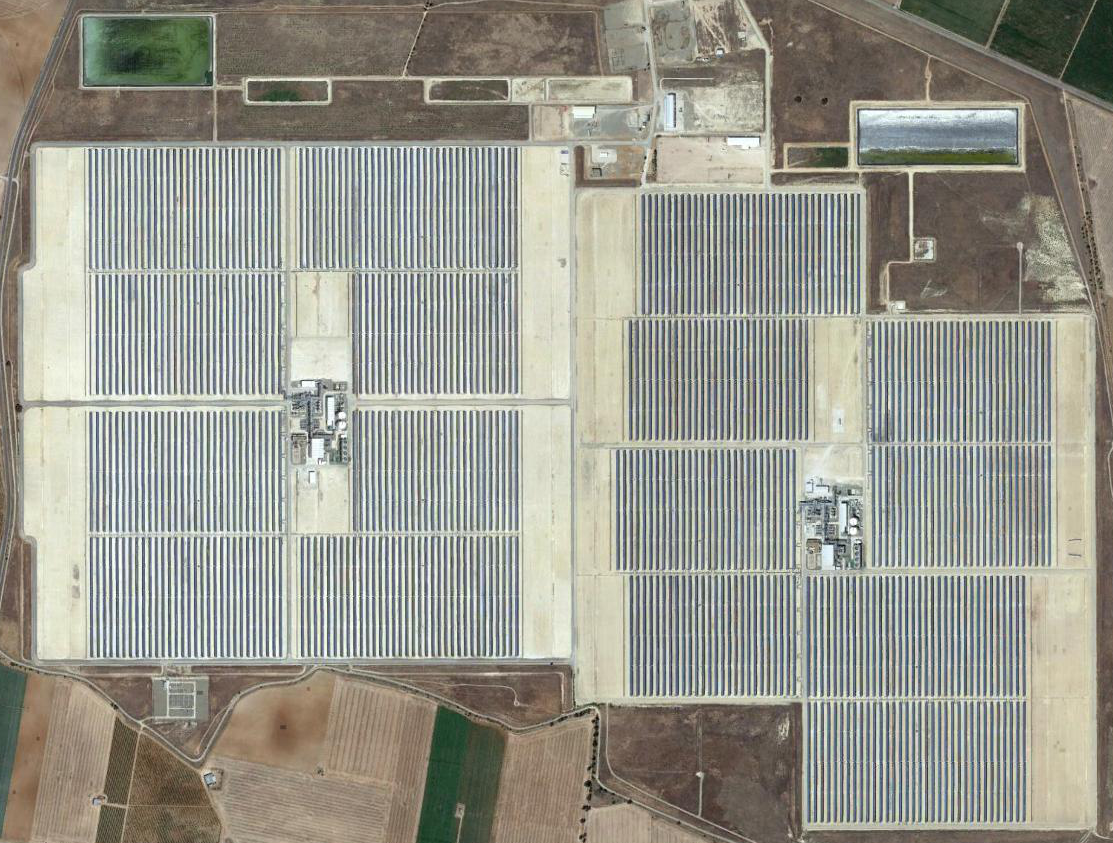
\includegraphics[width=0.9\linewidth]{images/fotoAstes.png}
\caption{Centrales Termosolares Aste 1A (izq.) y Aste 1B (der.) Fuente: Google Earth} 
\label{fig:astes}
\end{figure}

La potencia eléctrica nominal de cada una de ellas es de 49,9 MW. El proyecto inicial consideraba que las plantas contarían con almacenamiento térmico, el cual se construiría durante una segunda fase que finalmente no se llegó a ejecutar, por lo que en la actualidad solo existe generación durante las horas de sol. Se emplearán los datos de Aste 1B, cuya configuración es la siguente:

El campo solar cuenta con 120 lazos distribuidos de manera irregular en 4 subcampos. La  distancia de separación entre lazos es de 16,25 m. 

\begin{itemize}[itemsep=2pt,parsep=2pt]
\item
  Subcampo NO, 31 lazos.
\item
  Subcampo NE, 28 lazos.
\item
  Subcampo SO, 27 lazos.
\item
  Subcampo SE, 34 lazos.
\end{itemize}

Todos los lazos son idénticos, contando con 4 SCAs cada uno en una configuración tipo \(U\). El eje de seguimiento perfectamente plano se encuentra alineado en direccion N-S. Cada SCA cuenta con un total de 336 espejos de vídrio fabricados por Flabeg.

El fluido de trabajo es Dowtherm A, cuyas propiedades también se han descrito en el apartado \ref{subclases-fluid}.

Los datos meteorológicos son los recogidos a lo largo durante 2016 por las tres estaciones meteorológicas con las que cuenta la planta. Al tener por triplicado las medidas de cada variable se adopta el criterio de seleccionar la mediana de las tres y no el valor medio. Esta selección la realiza el sistema de control de planta en cada momento y con este criterio se persigue conseguir una mayor robustez del sistema, pues si una estación presenta valores muy desviados de las otras dos podría darse el caso de que el valor medio estuviese muy alejado del valor  verdadero. Cuando por avería o fallo de comunicación se carece de los datos de alguna estación sí se suele adoptar el criterio de seleccionar el valor medio de las dos restantes.

\subsection{Resultados de la simulación con Python}

Tras ejecutar la simulación compararemos los datos obtenidos de la simulación con los datos reales. 

 

